\subsection{Repartition Frequency}
The results of our repartition frequency experiments are shown in Figure \ref{fig:FrequencySensitivity}. We ran experiments using 8 partitions based on results from the partition count results, discussed in the Partition Count section. The experiments were run using 42,875 blocks on a single machine with 12 and 16 cores. The repartition frequency determines how often the RDD gets redistributed among the executor nodes to maintain load balance. As can be seen in the results, repartitioning more often generally leads to faster runs with a repartion period on the order ~15 discontinuities giving close to optimal performance. \par

There is a significant spike in the time it took the runs to complete when using a repartition period of 50 joints. This can be explained when considering the number of joints in the data set was 105 - the RDD was repartitioned twice during the computations and the last repartition occured when the calculations were almost completed and the RDD was close to its maximum size. Clearly, this is not a good time to repartition since the amount of data that has to be shuffled is close to the maximum value and the gains from load balancing will be short lived as the computations are nearly completed. \par

\begin{figure}
  \centering
  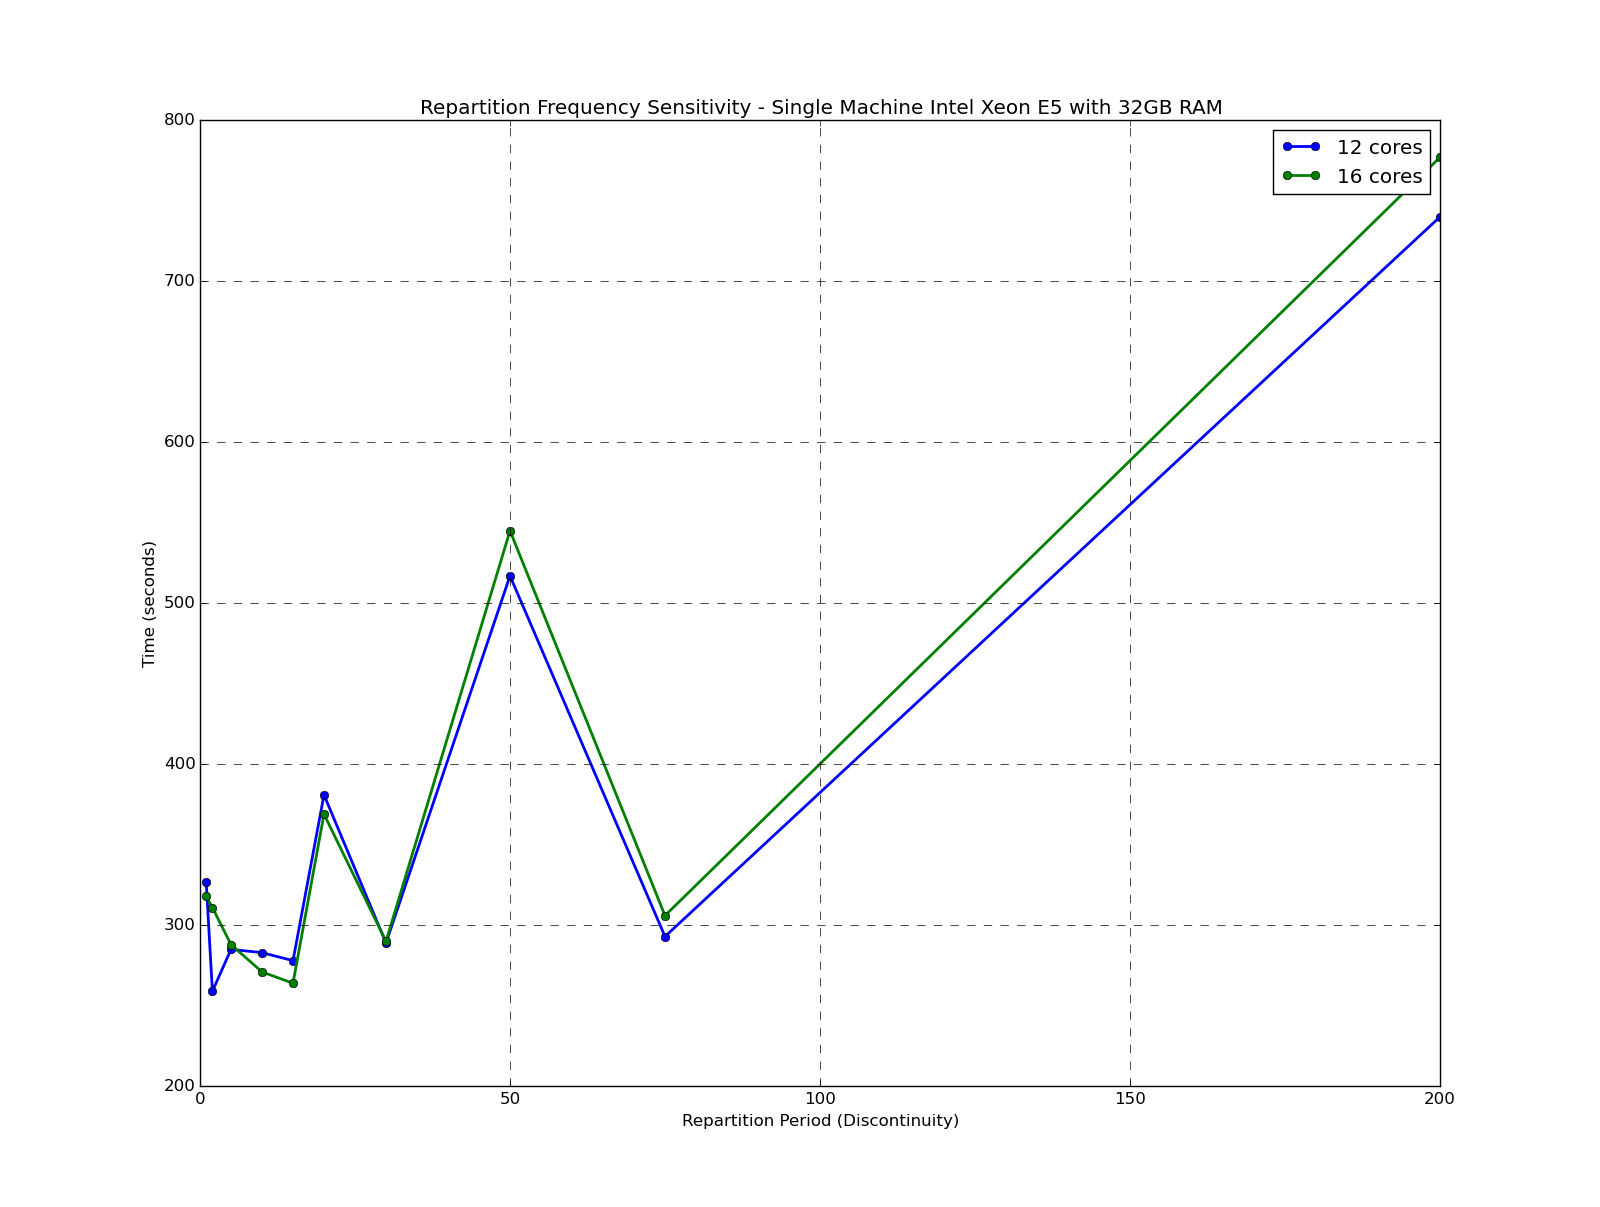
\includegraphics[width=0.4\textwidth]{FrequencySensitivity} 
  \label{fig:FrequencySensitivity}           
\end{figure}

Conversely, computation times close to optimal were achieved by repartitioning only once after 75 joints had been processed. This makes intuitive sense as it seems to strike a balance between minimizing shuffling  while  maintaining a balanced load. It is possible that as a ``rule of thumb'' repartitioning only once when approximately 75\% of the joints have been proccessed will give timings close enough to optimum for general use. Unfortunately, there was insufficient time to investigate this phenomenon further due to time constraints. \par

Lastly, the increased computation times at large repartition periods illustrate how load imbalance significantly deteriorates the efficiency of the computations. For our experiments, a repartition period of 200 implies that the RDD was not repartitioned at all since only 105 joints were processed. As previously discussed, this caused tremendous load-imbalance due to the nature of the input data set. \par

\subsection{Partition Count}
Figure \ref{fig:PartCount} shows the results of our sensitivity analysis for RDD partitioning. Tests were run using a repartition period of 15 joints - the results of the repartition frequency experiments indicated that this would be close to optimum for ~42,000 blocks. The results for number of partitions are somewhat counter intuitive - in both cases the best speeds were achieved by having less partitions than the number of cores. \cite{sparkTuning} recommends having more partitions than the number of cores as general rule to increase parallelism; however, this does not appear to be the case for our analysis. It is possible that in our case the tasks that need to be completed on each RDD are more time consuming since the cutting and intersection methods invoke a linear program solver for each joint that is processed. This could lead to long idle times for threads that end up taking a lot of memory and computational capacity away from the actual computations. More experimentation and a deeper understanding of how Spark manages RDD's and parallism is necessary to fully understand this behavior. \par

\begin{figure}
  \centering
  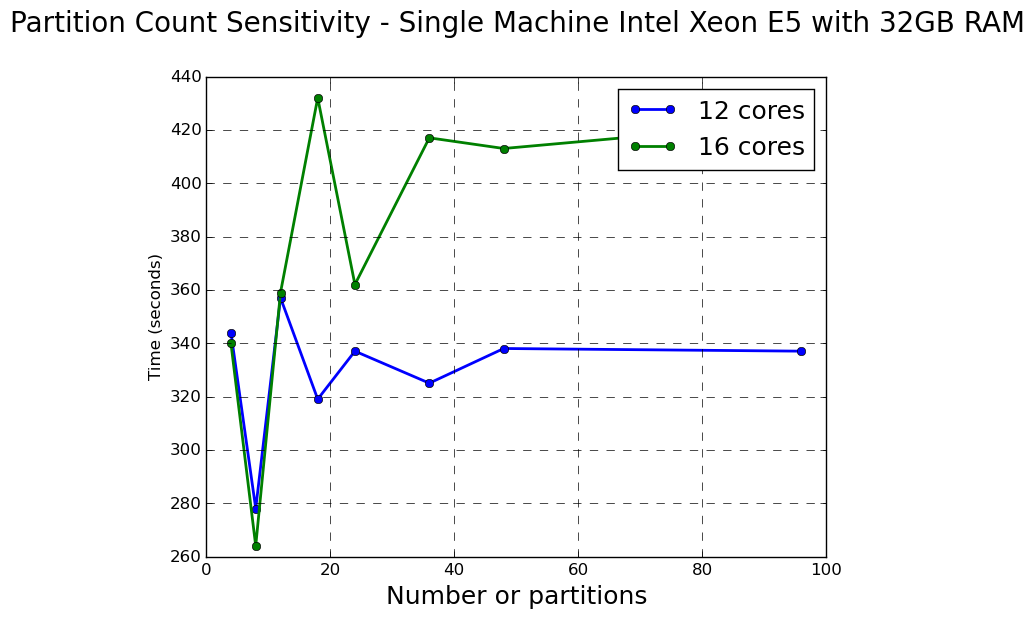
\includegraphics[width=0.4\textwidth]{PartCount} 
  \label{fig:PartCount}           
\end{figure}

What is clear from the experiments though is that getting the partition number wrong actually leads to worse performance when using more cores. Only by selecting the correct amount of partitions does it lead to increased performance for more computing power - 16 cores only outperformed 12 cores when using 8 partitions. For all other partition values tested 12 cores are faster than 16, especially when using more partitions.

\subsection{Weak Scaling}
\begin{figure*}[t]
\centering
\begin{subfigure}{0.5\textwidth}
    \centering
    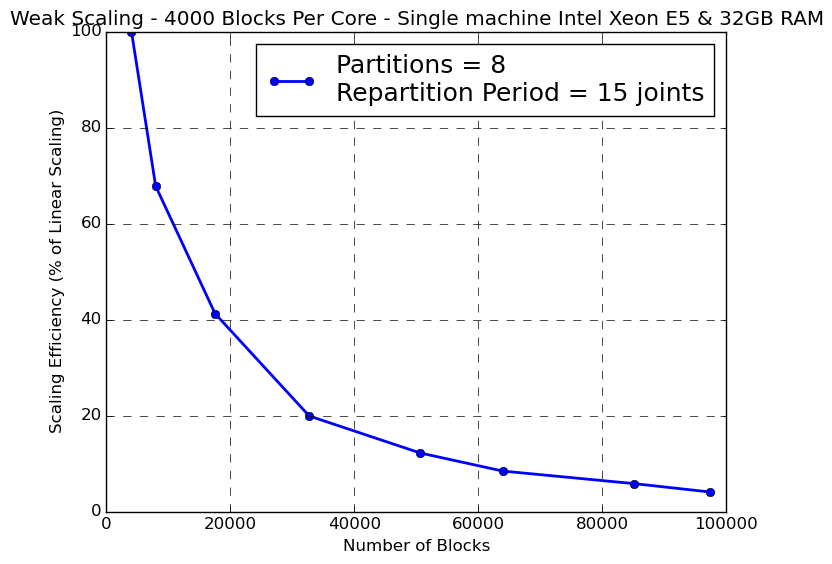
\includegraphics[width=0.4\textwidth]{weakScalingEfficiency.png}
    \caption{Efficiency Relative to Serial Execution}
\end{subfigure}%
\begin{subfigure}{0.5\textwidth}
    \centering
    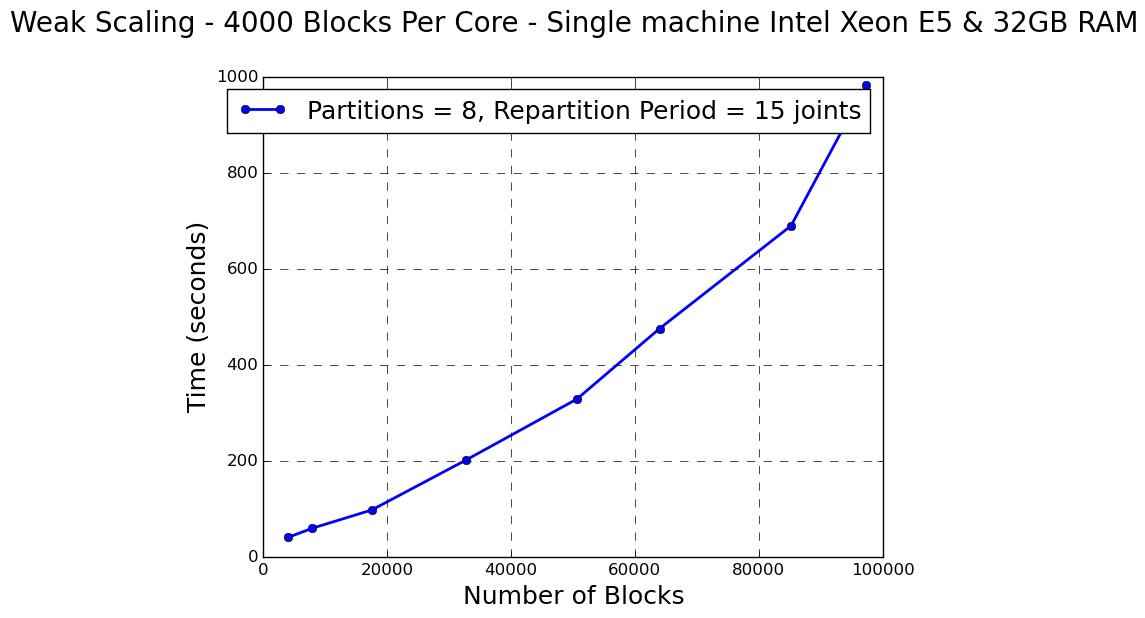
\includegraphics[width=0.4\textwidth]{weakScalingTime.png}
    \caption{Execution Time vs. Number of Cores}
\end{subfigure}
\caption{Weak Scaling Results when Processing 4000 Rock Blocks Per Core}
\label{fig:weakScaling}
\end{figure*}

The results from our evaluation of weak scaling are presented in Figure \ref{fig:weakScaling}. These show that the weak scaling of our implementation is actually rather poor. Our tests involved processing a rock mass containing roughly 4,000 rock blocks per CPU core. As can be seen in our graphs, the efficiency of our algorithm consistently diminishes as the number of cores increases. For example, once two cores are used to process 8,000 blocks, efficiency decreases to roughly 65\% of what was achieved when processing 4,000 blocks with just one core. What this means is that running our algorithm on an additional core incurs substantial overhead. We speculate that this is due to expensive communication amongst Spark workers and the data skew described in section 4. We ran these tests with eight partitions and using a repartition period of 15, based on the positive results using these parameter values in our previous experiments. However, it is likely that with more tuning and a better knowledge of Spark's internals, we can refactor our implementation to achieve much better weak scaling. We hope to accomplish this as part of our future work.

\subsection{Strong Scaling}
\begin{figure*}[t]
\centering
\begin{subfigure}{0.5\textwidth}
    \centering
    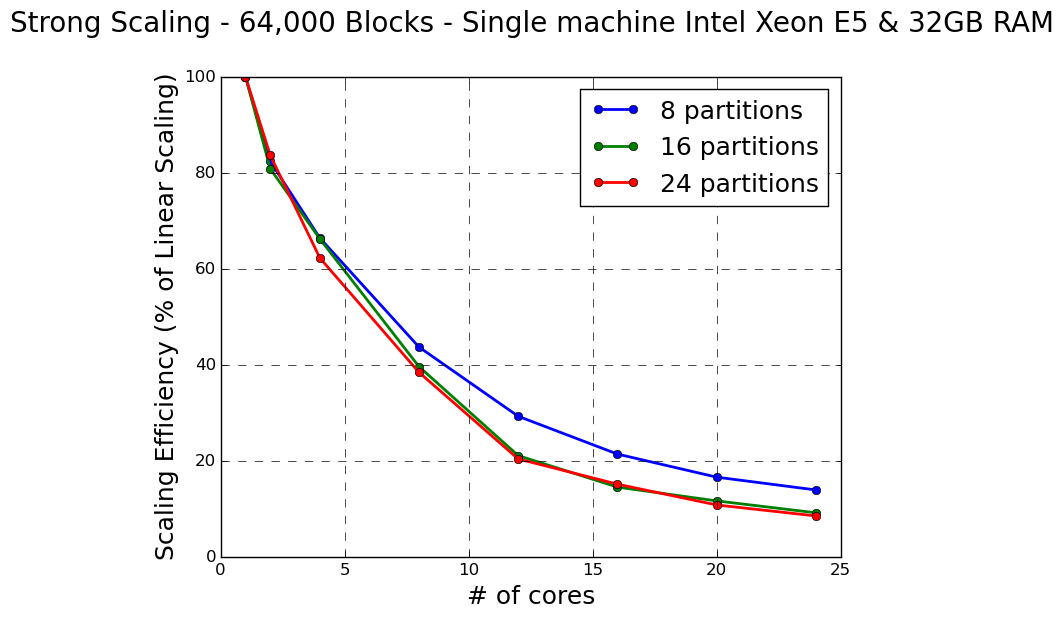
\includegraphics[width=0.4\linewidth]{strongScalingEfficiency.png}
    \caption{Efficiency Relative to Serial Execution}
\end{subfigure}%
\begin{subfigure}{0.5\textwidth}
    \centering
    \includegraphics[width=0.4\linewidth]{strongScaling.png}
    \caption{Execution Time vs. Number of Cores}
\end{subfigure}
\caption{Weak Scaling Results when Processing 4000 Rock Blocks Per Core}
\label{fig:strongScaling}
\end{figure*}

Our strong scaling results, presented in Figure \ref{fig:strongScaling}, are much more encouraging than the weak scaling results. We analyzed a rock mass containing 64,000 distinct blocks and again used a repartition frequency of 15 joints. Obviously to test strong scaling, we increased the number of cores that serve as Spark workers and observed the change in execution time. We repeated this experiment for three different RDD partition counts: 8, 16, and 24. Once again, we found that the 8-partition case yielded the best performance, confirming our partition count experiment described above. The shape of our graph conforms to our expectations: adding more cores to the Spark cluster does lead to better performance, but diminishing returns quickly emerge. The algorithm executes most quickly when it runs on 8 to 12 processors, and adding more cores beyond this point doesn't produce any benefit. In fact, partition count appears to determine the extent to which strong scaling can be achieved. For a partition count of 8, the execution time appears to level off once more than 12 processors are used, while for partition counts of 16 and 24 the execution time begins to increase past this point. Once again, we leave a more comprehensive investigation of this behavior to future work, and speculate that once we have a better understanding of the nuances of Spark, we may be able to make our algorithm more scalable.

\subsection{In Depth Profiling}
\begin{figure*}[t]
\centering
\begin{subfigure}{0.5\textwidth}
    \centering
    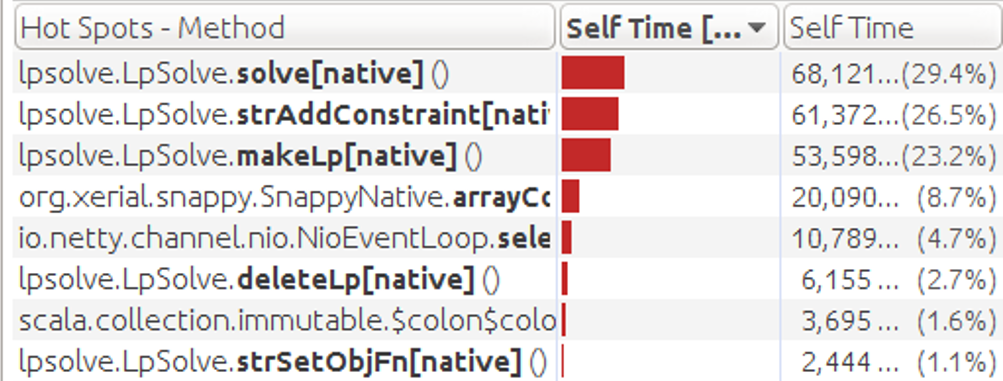
\includegraphics[width=0.4\linewidth]{visualVMComputation.png}
    \caption{Sample of Functions}
\end{subfigure}%
\begin{subfigure}{0.5\textwidth}
    \centering
    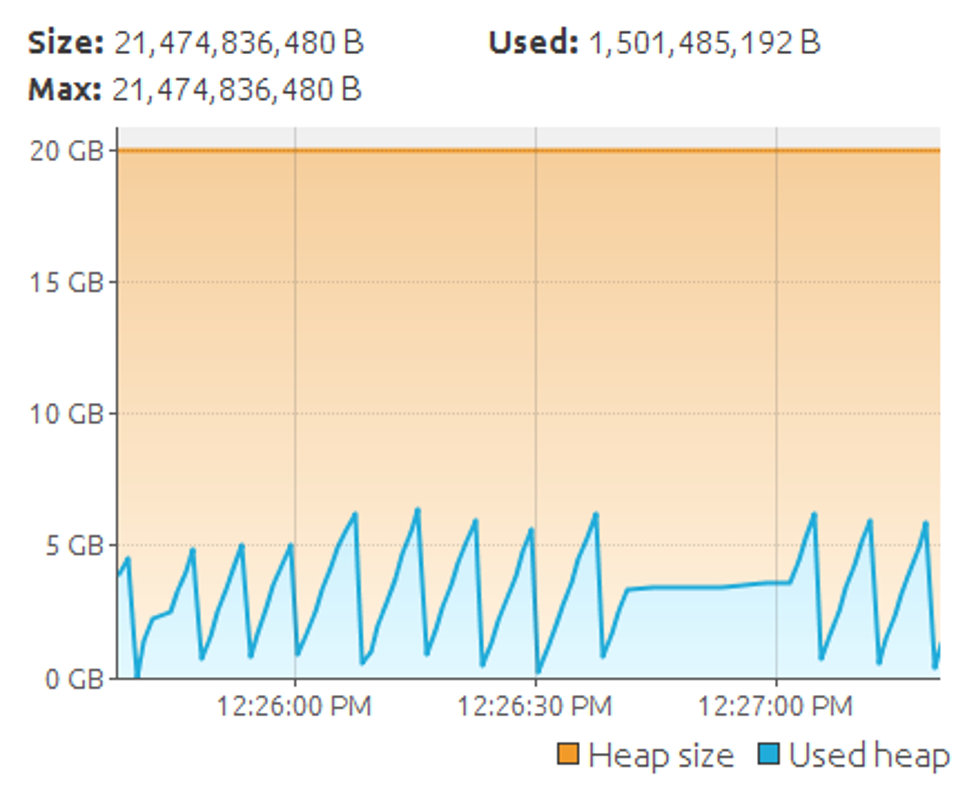
\includegraphics[width=0.4\linewidth]{visualVMMemory.png}
    \caption{Memory Behavior}
\end{subfigure}
\caption{Profiling Data From VisualVM}
\label{fig:visualVM}
\end{figure*}
We used the VisualVM Java profiler \cite{visualVM} in order to gain a clearer picture of the behavior of our algorithm on Spark. We were interested in two main questions: 1) Which computations dominate the execution time of our algorithm? and 2) What are the memory consumption patterns of our algorithm? The results produced by VisualVM are shown in Figure \ref{fig:visualVM}. The first subfigure shows function sampling results from a typical execution of our algorithm. These results indicate that the majority of execution time is spent constructing and solving linear programs. This is an encouraging sign, as it implies that increased parallelism has the potential to speed up the rock slicing process. This is one of the reasons why we speculate that we will be able to improve the performance of our slicing algorithm once we are able to make a more effective use of Spark.

The second subfigure shows the memory consumption of the rock slicing algorithm over time. The jagged shape of this graph is caused by periods of gradual in-memory data accumulation as processing occurs followed by executions of Java's garbage collector to reduce memory consumption. This could indicate that garbage collection plays a role in some of the performance issues we have observed in previous experiments. Clearly, more experimentation will be needed to fully understand the memory usage patterns of our algorithm and potential improvements to the implementation to improve its memory behavior.
